\documentclass{article}

\usepackage{graphicx} % Required for inserting images
\usepackage{amsmath}
\usepackage{biblatex}
\addbibresource{reference.bib}

\title{A Review of Geometric Algebra in Signal and Image Processing.}
\author{Tanvir Jahan Alin}
\date{01 November, 2023}

\begin{document}

\maketitle

\begin{abstract}

Recently, Geometric Algebra (GA) has attracted more and more attention in the field of signal
and image processing. GA can treat multi-dimensional signals in a holistic way to keep the correlations
among multiple dimensions and avoid information loss. So when traditional signal and image processing
algorithms are redefined in GA space, they will be more powerful and achieve better performance in
multi-dimensional signal processing. In this paper, we provide a comprehensive survey covering various
GA-based algorithms. In particular, we first review the mathematic theories of GA and Reduced Geometric Algebra. Then, advanced GA-based algorithms are elaborately analyzed and compared, including GA-based Sparse representation model, GA-based Dictionary Learning method, Clifford Support Vector Machine, GA-based Feature extraction algorithms, GA-based adaptive filtering algorithms, GA-based
Fourier-type transform, and GA-based edge detection algorithm. Finally, we discuss several open issues
and challenges of GA, and point out possible research directions in the future.
  
\end{abstract}

\section{Introduction}
Geometric algebra (GA) has been considered as one of the
most powerful tools in mathematics and has witnessed great
success in a wide range of applications, such as physics, quantum computing, electromagnetism, satellite navigation, neural computing, camera geometry, image processing, robotics
and computer vision, etc. The above-mentioned application
fields are reviewed in 2013 [1]. Since it is impossible to make
a complete overview for the enormous range of applications
developed in the past decades, particularly, we try to give an
overview on theory and applications of GA mainly in signal
and image processing.
\newline
For multi-channel signals, traditional methods usually
treat each channel as a different vector and process them
independently, which may fail to exploit the correlations
among multiple channels and lead to information loss. Fortunately, GA can transform multi-dimensional signals into
multivectors and handle them in a holistic manner in a
new multi-dimensional GA space

\section{RELATED WORK }
\subsection{THE BASIC OF GEOMETRIC ALGEBRA }
Geometric algebra (GA)\cite{sommer2013geometric}\cite{wang2019l1} is created by W.K. Clifford, also called Clifford algebra. GA provides a mathematical framework, which is ideal to constitute an extension of real, complex and quaternion algebras to complete associative algebras of subspaces of vector spaces in the general framework of vector. \\

The addition of GA can be defined as 
\begin{table}
    \centering
    \begin{tabular}{|c|c|} \hline 
        \begin{equation}
e^2_{a\i} =1
\end{equation}& \begin{equation}
e^2_{a\i} =-1
\end{equation}\\ \hline 
        
    \end{tabular}
    \caption{equation}
    \label{tab:my_label}
\end{table}



\subsection{ APPLICATIONS TO SIGNAL AND IMAGE PROCESSING}

For image processing, the sparse representation model based
on dictionary learning plays an important role. Taking advantages of the sparse representation, a color image can be
well-represented as a sparse linear combination of elements
from an appropriately chosen over-complete dictionary,
rather than being separated into independent components.
The singular value decomposition (SVD), as the most popular method for sparse representation, have recently attracted
intensive interest and achieved great success. Since pure virtual quaternion can be perfectly embedded the spectral data
of RGB channel of color image, the spectral information and
spatial information of color image can be fully explored by
quatern

\begin{figure}[h]
        \centering
        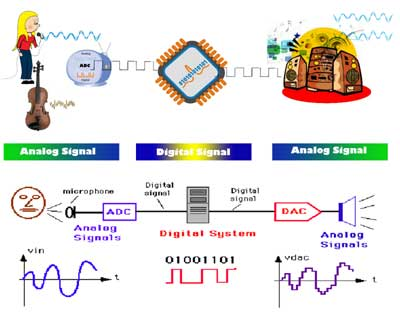
\includegraphics[width=0.5\textwidth]{signalprocessing.jpg}
        \caption{Signal and image processing}
        \label{fig:enter-label}
    \end{figure}

\section{Example}
Signal and image processing are fundamental in various fields, including telecommunications, medical imaging, and computer vision. Here's an example of each:

\subsection{Signal Processing:}
Consider a mobile phone receiving a voice call. The audio signal picked up by the microphone is a continuous analog signal. To transmit this signal efficiently and without distortion, it needs to be processed. This involves converting the analog signal to a digital one through analog-to-digital conversion. Digital signal processing techniques are then applied to remove noise, compress the data, and enhance voice clarity. The processed digital signal is transmitted, received, and converted back to analog for the listener.

\subsection{Image Processing:}
In the field of medical imaging, consider a digital X-ray image of a patient's chest. Image processing techniques are employed to enhance the visibility of specific features, such as bones or soft tissues. Filters can be applied to reduce noise and improve the image's contrast. Edge detection algorithms can help identify boundaries of structures, and computer vision methods can be used for automatic diagnosis, like identifying potential fractures or abnormalities.

Both signal and image processing play crucial roles in extracting meaningful information from data, enhancing quality, and enabling automation in various applications.

\section{Conclusion}
In conclusion, this paper presents a comprehensive review on GA in signal and image processing. The application of GA has been summarized, with the analysis of their advantages and shortcomings. Also, the challenges and prospects of various applications proposed by many researchers have been given. With continuous developments in computer vision field and the improvement of computer hardware performance, we believe that the existing problems can be solved step by step via GA-based algorithms. And it is expected that the GA-based theories and algorithms will be a competitive alternative in applications of signal and image processing. 





\printbibliography

\end{document}
